\documentclass{beamer}

\usetheme{Warsaw}
\usecolortheme{crane}

\usepackage[utf8]{inputenc}
\usepackage[english]{babel}
\usepackage{xcolor}
\usepackage{listings}
\lstset{%
  basicstyle=\ttfamily\footnotesize,
  showstringspaces=false,
  escapeinside={<@}{@>}
}

\graphicspath{{images/}}
\title[Intro to Git]{Introduction to Git}

\author{Armin Leuprecht}
\institute
{
  Wegener Center for Climate and Global Change\\
  University of Graz
}
\date[2016-07-28]{T4S, 28$^{th}$ July 2016}

% \AtBeginSection[]
% {
%   \begin{frame}
%     \frametitle{Table of Contents}
%     \tableofcontents[currentsection]
%   \end{frame}
% }


\begin{document}
\beamertemplatenavigationsymbolsempty

\begin{frame}
  \titlepage
\end{frame}

\section[VCSs]{Version control systems}
\begin{frame}
  \frametitle{Version control}
  \framesubtitle{Record the history of files}

  Why do you want to use a VCS?
  \begin{itemize}
  \item revert to previous file versions
  \item compare changes over time
  \item find out who modified something
  \item easy recovery when things screw up
  \end{itemize}

  Why do you have to use a VCS?
  \begin{itemize}
    \item reproducibility
    \item transparency
    \item confirmability
  \end{itemize}
\end{frame}

\begin{frame}[fragile]
  \frametitle{Types of VCSs}
  \begin{itemize}
  \item<1-> Manual version control
  \item<2-> Local VCS
  \item<3-> Centralized VCS
  \item<4-> Distributed VCS
  \end{itemize}

  \begin{overprint}
    \onslide<1>
    \begin{alertblock}{Manual VC}
      \emph{No good idea -- very error prone}
      \begin{lstlisting}[language=bash]
        ...
        v179_20150115_ReLoClimWrittenPublications.docx
        v180_20150115_ReLoClimWrittenPublications.docx
        v180b_20150115_ReLoClimWrittenPublications.docx
        v181_20150205_ReLoClimWrittenPublications.docx
        v182_20150205_ReLoClimWrittenPublications.docx
        v183_20150206_ReLoClimWrittenPublications.docx
      \end{lstlisting}
    \end{alertblock}

    \onslide<2>
    \begin{block}{Local CSV}
      \begin{minipage}{.5\linewidth}
        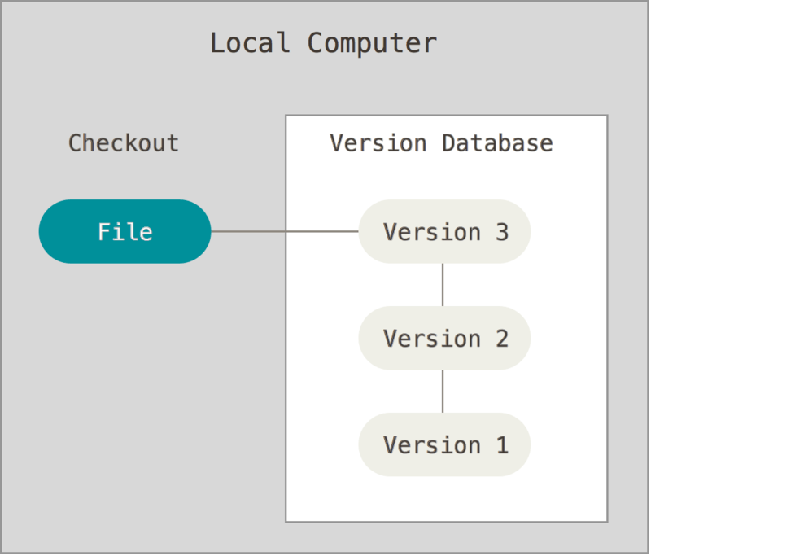
\includegraphics[width=\textwidth]{local}        
      \end{minipage}\hfill
      \begin{minipage}{.5\linewidth}\small
        Pros:
        \begin{itemize}
          \item fast and easy for single user/machine
        \end{itemize}
        Cons:
        \begin{itemize}
          \item difficult administration over systems
        \end{itemize}
        Examples: rcs
      \end{minipage}

    \end{block}

    \onslide<3>
    \begin{block}{Centralized VCS}
      \begin{minipage}{.5\linewidth}
        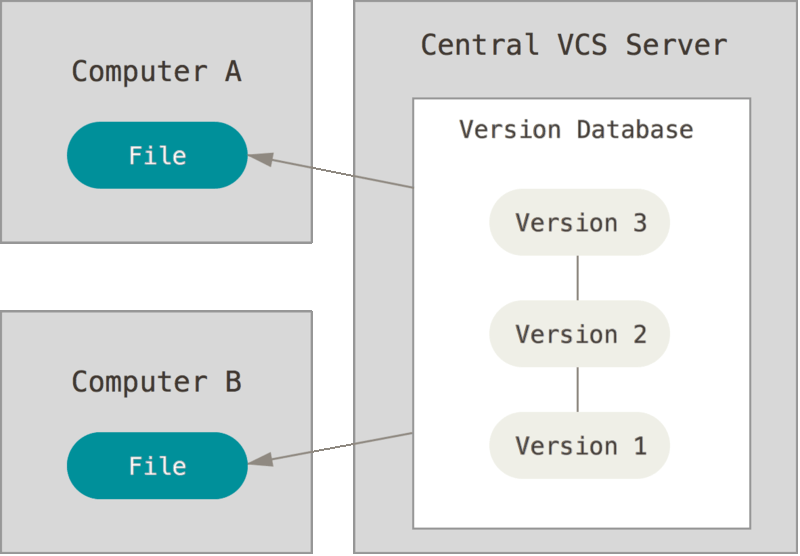
\includegraphics[width=\textwidth]{centralized}
      \end{minipage}
      \begin{minipage}{.45\linewidth}\small
        Pros:
        \begin{itemize}
          \item easy administration
          \item fine-grained control
        \end{itemize}
        Cons:
        \begin{itemize}
          \item single point of failure
        \end{itemize}
        Examples: cvs, subversion
      \end{minipage}
    \end{block}

    \onslide<4>
    \begin{exampleblock}{Distributed VCS}
      \begin{minipage}{.5\linewidth}
        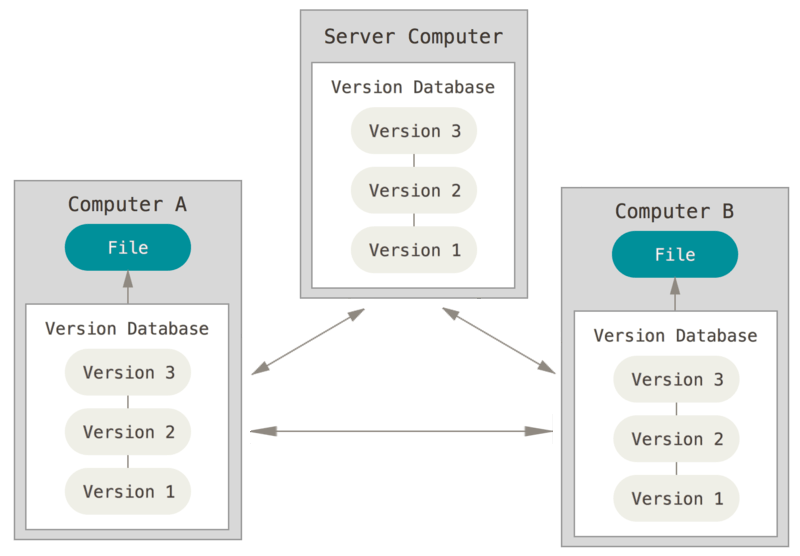
\includegraphics[width=\textwidth]{distributed}
      \end{minipage}
      \begin{minipage}{.45\linewidth}\small
        Pros:
        \begin{itemize}
          \item extremely fast
          \item full mirror of the repository
          \item several workflows
        \end{itemize}
        Cons:
        \begin{itemize}
        \item large binary files/history
        \end{itemize}
        Examples: Git, Mercurial, Bazaar
      \end{minipage}
    \end{exampleblock}

  \end{overprint}
    
\end{frame}

\section[Git Basics]{Git Basics}
\begin{frame}
  \frametitle{History}
  Created in 2005 for the development of the Linux kernel

  Naming (by Linux Torvalds) -- depending on your mood
  \begin{itemize}
    \item random three-letter combination that is pronounceable, and not
      actually used by any common UNIX command.  The fact that it is a
      mispronunciation of "get" may or may not be relevant.
    \item stupid. contemptible and despicable. simple. Take your pick from the
      dictionary of slang.
    \item "global information tracker": you're in a good mood, and it actually
      works for you. Angels sing, and a light suddenly fills the room.
    \item "goddamn idiotic truckload of sh*t": when it breaks
  \end{itemize}
\end{frame}

\begin{frame}
  \frametitle{Goals}
  \begin{itemize}
    \item Speed
    \item Simple design
    \item Fully distributed
    \item Emphasis on non-linear development
  \end{itemize}
\end{frame}

\begin{frame}[fragile]
  \frametitle{Storage: Snapshots -- no diffs}
  \begin{itemize}
    \item<1-> Traditional view: list of file-based deltas
    \item<2->   Git: stream of snapshots
      \begin{itemize}
        \item more like a mini file-system
        \item very efficient when it comes to branching
      \end{itemize}
  \end{itemize}

  \centering
  \begin{overprint}
    \onslide<1>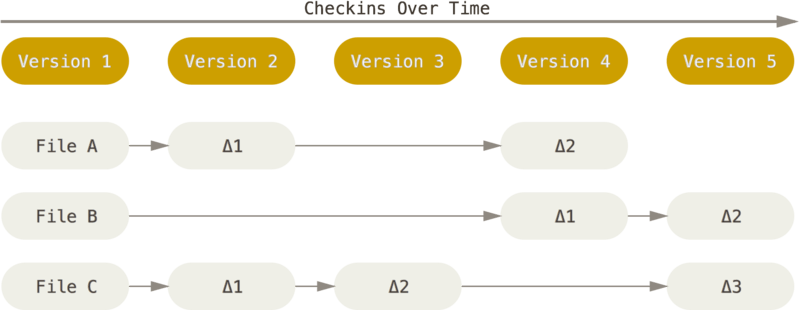
\includegraphics[width=.9\textwidth]{deltas}
    \onslide<2>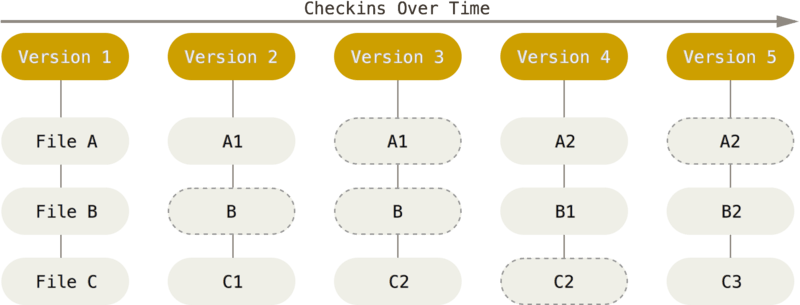
\includegraphics[width=.9\textwidth]{snapshots}
  \end{overprint}
\end{frame}

\begin{frame}
  \frametitle{Further advantages}
  \begin{itemize}
    \item Speed: nearly every operation is local
    \item Integrity: everything is checksummed
    \item Data loss: after commit and push nearly impossible
  \end{itemize}
\end{frame}

\begin{frame}
  \frametitle{The three stages}
  Every controlled file resides in one of three main states:
  \begin{itemize}
    \item modified: you have changed the file and not committed yet
    \item staged: you have marked the file to go into your next commit snapshot
    \item committed: data is safely stored in your local database
  \end{itemize}
\end{frame}

\begin{frame}
  \frametitle{Git workflow}
  \centering
  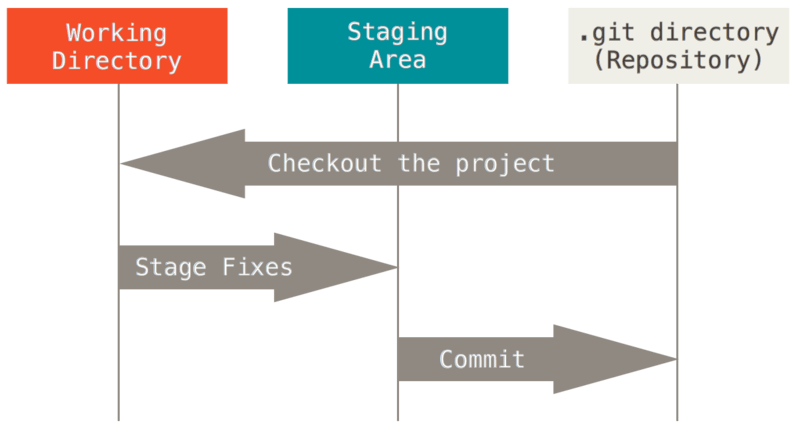
\includegraphics[width=.9\textwidth]{areas}
  \begin{itemize}
    \item modify files in working directory
    \item stage files (adding snapshots to the staging area)
    \item commit files (storing snapshots permanently in the Git directory)
  \end{itemize}
\end{frame}

\begin{frame}[fragile]
  \frametitle{Installation}
  \begin{itemize}
    \item your OS package manager (apt, yum)
    \item binary packages from Git homepage download section: \url{https://git-scm.com/downloads}
    \item get it via Git and compile it on your own (if you already have a running version):\\ 
      \lstinline{git clone} \url{https://github.com/git/git}
  \end{itemize}
\end{frame}

\begin{frame}[fragile]
  \frametitle{First-time setup}
  There are three configuration places
  \begin{itemize}
    \item \lstinline{/etc/gitconfig} file: system-wide for any user (written by superuser only)
    \item \lstinline{~/.gitconfig} or \lstinline{~/.config/git/config} file: specific to the user, can be accessed by passing the \lstinline{--global} option to \lstinline{git config}
    \item \lstinline{config} file in the Git directory (\lstinline{.git/config}): specific to that repository
  \end{itemize}

  Setup your identity (and your prefered editor)
  \begin{lstlisting}[language=bash]
    $ git config --global user.name "Jane Doe"
    $ git config --global user.email jane.doe@example.com

    $ git config --global core.editor emacs
  \end{lstlisting}
\end{frame}

\begin{frame}[fragile]
  \frametitle{Getting help}
  Besides many resources on the web you will get (offline) help by calling the manual pages:

  \begin{lstlisting}[language=bash]
    $ git help <verb>
    $ git <verb> --help
    $ man git-<verb>
  \end{lstlisting}

  Example: 
  \begin{lstlisting}[basicstyle=\ttfamily\tiny]
$ git help commit
GIT-COMMIT(1)                       Git Manual                    GIT-COMMIT(1)

NAME
       git-commit - Record changes to the repository

SYNOPSIS
       git commit [-a | --interactive | --patch] [-s] [-v] [-u<mode>] [--amend]
                  [--dry-run] [(-c | -C | --fixup | --squash) <commit>]
                  [-F <file> | -m <msg>] [--reset-author] [--allow-empty]
                  [--allow-empty-message] [--no-verify] [-e] [--author=<author>]
                  [--date=<date>] [--cleanup=<mode>] [--[no-]status]
                  [-i | -o] [-S[<key-id>]] [--] [<file>...]

...
  \end{lstlisting}
\end{frame}

\begin{frame}[fragile]
  \frametitle{Getting a repository}
  Initialize a repo in an existing directory
  \begin{lstlisting}[language=bash]
    $ git init .

    $ git add *.py
    $ git add README.md
    $ git commit -m 'initial commit'
  \end{lstlisting}

  Cloning an existing repo
  \begin{lstlisting}[language=bash]
    $ git clone https://github.com/django/django.git
  \end{lstlisting}
  Other protocols: ssh, git
\end{frame}

\begin{frame}
  \frametitle{Lifecycle of your files in the repo}
  \centering
  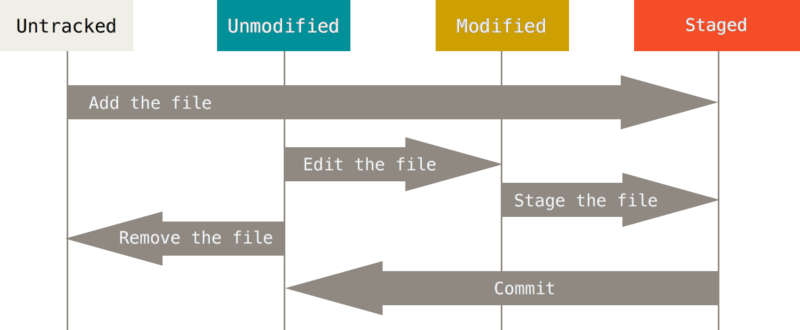
\includegraphics[width=.9\textwidth]{lifecycle}
\end{frame}

\begin{frame}[fragile]
  \frametitle{Checking status of your files}

  Checking
  \begin{lstlisting}[language=bash,basicstyle=\ttfamily\tiny]
    $ git status
    On branch basics
    Changes not staged for commit:
      (use "git add <file>..." to update what will be committed)
      (use "git checkout -- <file>..." to discard changes in working directory)

           <@\textcolor{red}{modified:   git.tex}@>

    Untracked files:
      (use "git add <file>..." to include in what will be committed)

           <@\textcolor{red}{images/lifecycle.png}@>

    no changes added to commit (use "git add" and/or "git commit -a")
  \end{lstlisting}

  Add the image
  \begin{lstlisting}[language=bash,basicstyle=\ttfamily\tiny]
    $ git add images/lifecycle.png
  \end{lstlisting}
\end{frame}

\begin{frame}[fragile]
  \frametitle{Checking status of your files}
  Rechecking
  \begin{lstlisting}[language=bash,basicstyle=\ttfamily\tiny]
    $ git status
    On branch basics
    Changes to be committed:
      (use "git reset HEAD <file>..." to unstage)

           <@\textcolor{green}{new file:   images/lifecycle.png}@>

    Changes not staged for commit:
      (use "git add <file>..." to update what will be committed)
      (use "git checkout -- <file>..." to discard changes in working directory)

           <@\textcolor{red}{modified:   git.tex}@>

  \end{lstlisting}

  Short output using \lstinline{-s} or \lstinline{--short}
  \begin{lstlisting}[language=bash,basicstyle=\ttfamily\tiny]
    $ touch emptyfile
    $ git status --short
     <@\textcolor{red}{M}@> git.tex
    <@\textcolor{green}{A}@>  images/lifecycle.png
    <@\textcolor{red}{??}@> emptyfile

    $ rm emptyfile
  \end{lstlisting}
\end{frame}

\begin{frame}[fragile]
  \frametitle{Ignoring files}
  Files you do not want to track at all
  \begin{lstlisting}[language=bash,basicstyle=\ttfamily\tiny]
    $ cat .gitignore
    *~
    *.pdf
    *.log
    *.out
    *.aux
    *.nav
    *.snm
    *.toc
    *.vrb
    .#*
    \#*#
  \end{lstlisting}

  \begin{itemize}
    \item standard glob patterns
    \item starting with a slash \lstinline{/} avoids recursivity
    \item ending with a slash \lstinline{/} denotes directories
    \item negate the pattern with an exclamation mark \lstinline{!}
    \item two asterisks between slashes \lstinline{/**/} matches nested dirs
  \end{itemize}
\end{frame}

\begin{frame}[fragile]
  \frametitle{Viewing your changes}
  Use \lstinline{git diff} to see the changes between changed but not staged file
  \begin{lstlisting}[language=bash,basicstyle=\ttfamily\tiny,escapeinside={<!}{!>}]
    $ git diff git.tex

    diff --git a/git.tex b/git.tex

    index 336c02b..911eed3 100644
    --- a/git.tex
    +++ b/git.tex
    <!\textcolor{cyan}{@@ -5,16 +5,17 @@}!>
 
     \usepackage[utf8]{inputenc}
     \usepackage[english]{babel}
    <!\textcolor{red}{-}!>
    <!\textcolor{green}{+{\textbackslash}usepackage\{xcolor\}}!>
      \usepackage{listings}
      \lstset{%
        basicstyle=\ttfamily\footnotesize,
        showstringspaces=false,
    <!\textcolor{green}{+}!>   <!\textcolor{green}{escapeinside=\{<@\}\{@>\}}!>
     }
     ...
  \end{lstlisting}

  Use \lstinline{git diff --staged} to see the diff between a staged file and your last commit

\end{frame}

\begin{frame}[fragile]
  \frametitle{Committing your changes}
  A simple \lstinline{git commit} will commit all your staged files.

  \begin{lstlisting}[basicstyle=\ttfamily\tiny]
    $ git commit -m 'Added the lifecycle image'
    [basics c840fed] Added the lifecycle image
    1 file changed, 0 insertions(+), 0 deletions(-)
    create mode 100644 images/lifecycle.png
  \end{lstlisting}

  Caution: \lstinline{git commit -a} skips the explicitly staging of files
  and commits every modified file immediately.
\end{frame}

\begin{frame}[fragile]
  \frametitle{Removing files}
  To remove a file completely you remove it from the staging area and then you commit
  \begin{lstlisting}[basicstyle=\ttfamily\tiny]
    $ git rm somefile
    $ git commit -m 'removal of somefile'
  \end{lstlisting}
  This will also remove it from your working directory.

  To remove a file from the staging area but keep it in your working directory
  use \lstinline{git rm --cached somefile}
\end{frame}

\begin{frame}[fragile]
  \frametitle{Moving files}
  Git does not explicitly track file movement. Thus there is a \lstinline{git mv} command
  \begin{lstlisting}[basicstyle=\ttfamily\tiny]
    $ git mv git.tex presentation.tex
    $ git status
    On branch basics
    Changes to be committed:
      (use "git reset HEAD <file>..." to unstage)

            <@\textcolor{green}{renamed:}@>    <@\textcolor{green}{git.tex -> presentation.tex}@>

    Changes not staged for commit:
    (use "git add <file>..." to update what will be committed)
      (use "git checkout -- <file>..." to discard changes in working directory)

            <@\textcolor{red}{modified:}@>    <@\textcolor{red}{presentation.tex}@>
  \end{lstlisting}
\end{frame}

\begin{frame}[fragile]
  \frametitle{Viewing history}
  View the log of the commits
  \begin{lstlisting}[basicstyle=\ttfamily\tiny]
    $ git log
    <@\textcolor{orange}{commit c840fed176e56dc2b25145be8f12b779a1b1a402}@>
    Author: Armin Leuprecht <armin.leuprecht@uni-graz.at>
    Date:   Wed Jul 27 15:19:53 2016 +0200

        Added the lifecycle image

    <@\textcolor{orange}{commit dc36e922bb536e3b79406e7612ce74095cab0221}@>
    Author: Armin Leuprecht <armin.leuprecht@uni-graz.at>
    Date:   Tue Jul 26 16:25:17 2016 +0200

        initial commit -- basic slides
  \end{lstlisting}

  \lstinline{git log -p -2} shows diffs and limits output to the last two commits

  There are many command-line switches, just look at \lstinline{git log --help}
\end{frame}

\begin{frame}[fragile]
  \frametitle{Undoing things}
  When you forgot to add a file to the staging area before commit
  \begin{lstlisting}[basicstyle=\ttfamily\tiny]
    $ git commit --amend
  \end{lstlisting}

  Unstaging a file
  \begin{lstlisting}[basicstyle=\ttfamily\tiny]
    $ touch file
    $ git add file
    $ git status
    On branch basics
    Changes to be committed:
      (use "git reset HEAD <file>..." to unstage)

        <@\textcolor{green}{new file:}@>   <@\textcolor{green}{file}@>

    $ git reset HEAD file
    $ git status
    On branch basics
    Untracked files:
      (use "git add <file>..." to include in what will be committed)

        <@\textcolor{red}{file}@>

    $ rm file
  \end{lstlisting}
\end{frame}

\begin{frame}[fragile]
  \frametitle{Undoing things}
  Unmodify a modified file
  \begin{lstlisting}[basicstyle=\ttfamily\tiny]
    $ git status
    On branch basics
    Changes not staged for commit:
    (use "git add <file>..." to update what will be committed)
      (use "git checkout -- <file>..." to discard changes in working directory)

	    <@\textcolor{red}{modified:}@>    <@\textcolor{red}{presentation.tex}@>
    
    $ git checkout -- presentation.tex
    $ git status
    On branch basics
    nothing to commit, working directory clean
  \end{lstlisting}
  This would not be very wise as all changes are gone -- including this line

  If you want to  keep the changes but revert to a previous state you will need to branch $ldots$
\end{frame}

\begin{frame}[fragile]
  \frametitle{Remotes -- collaboration}
  Showing remotes
  \begin{lstlisting}[basicstyle=\ttfamily\tiny]
    $ git clone https://github.com/schacon/ticgit
    Cloning into 'ticgit'...
    remote: Reusing existing pack: 1857, done.
    remote: Total 1857 (delta 0), reused 0 (delta 0)
    Receiving objects: 100% (1857/1857), 374.35 KiB | 268.00 KiB/s, done.
    Resolving deltas: 100% (772/772), done.
    Checking connectivity... done.
    $ cd ticgit
    $ git remote
    origin
  \end{lstlisting}

  Including the verbose switch \lstinline{-v}
  \begin{lstlisting}[basicstyle=\ttfamily\tiny]
    $ git remote -v
    origin	https://github.com/schacon/ticgit (fetch)
    origin	https://github.com/schacon/ticgit (push)
  \end{lstlisting}
\end{frame}

\begin{frame}[fragile]
  \frametitle{Remotes -- adding remotes}
  Add a new remote explicitly
  \begin{lstlisting}[basicstyle=\ttfamily\tiny]
    $ git remote add pb https://github.com/paulboone/ticgit
    $ git remote -v
    origin      https://github.com/schacon/ticgit (fetch)
    origin      https://github.com/schacon/ticgit (push)
    pb          https://github.com/paulboone/ticgit (fetch)
    pb          https://github.com/paulboone/ticgit (push)
  \end{lstlisting}
  Now you are able to fetch Paul's information
  \begin{lstlisting}[basicstyle=\ttfamily\tiny]
    $ git fetch pb
    remote: Counting objects: 43, done.
    remote: Compressing objects: 100% (36/36), done.
    remote: Total 43 (delta 10), reused 31 (delta 5)
    Unpacking objects: 100% (43/43), done.
    From https://github.com/paulboone/ticgit
     * [new branch]      master     -> pb/master
     * [new branch]      ticgit     -> pb/ticgit
  \end{lstlisting}

  You now have local access to Paul's master branch as \lstinline{pb/master}
\end{frame}

\begin{frame}[fragile]
  \frametitle{Pulling and pushing} 
  Getting (fetch/pull)
  \begin{itemize}
    \item   Fetching by
      \lstinline{git fetch [remote-name]} downloads all data to you local
      repository since last clone/fetch/pull.
    \item   If your current branch is set up to track a remote branch (which is
      automatically done by the \lstinline{clone} command) you can do a
      \lstinline{git pull} to download and merge the remote branch into
      your local branch.
  \end{itemize}

  Sharing (push)
  
  When you have done your work (that you wanna share) you will use
  \lstinline{git push [remote-name] [branch-name]} to push your changes upstream.

  E.g. \lstinline{git push origin master} pushes your local master
  branch to the `orignal` remote (you've cloned from)
\end{frame}

\begin{frame}[fragile]
  \frametitle{Info on remotes}
  Inspect remote branches
  \begin{lstlisting}[basicstyle=\ttfamily\tiny]
    $ git remote show origin 
    * remote origin
      Fetch URL: git@github.com:wegener-center/zot2mail.git
      Push  URL: git@github.com:wegener-center/zot2mail.git
      HEAD branch: master
      Remote branch:
        master                 tracked
        dev-branch             tracked
      Local branch configured for 'git pull':
        dev-branch merges with remote dev-branch
        master     merges with remote master
      Local ref configured for 'git push':
        dev-branch         pushes to dev-branch   (up to date)
        master             pushes to master       (up to date)
  \end{lstlisting}
\end{frame}

\begin{frame}[fragile]
  \frametitle{Renaming and removing remotes}
  Changing the shortname of a remote:
  \begin{lstlisting}[basicstyle=\ttfamily\tiny]
    $ git remote rename pb paul
    $ git remote
    origin
    paul
  \end{lstlisting}
  this renames also your remote-tracking branch names: \lstinline{pb/master} becomes \lstinline{paul/master}

  If you want to remove a remote:
  \begin{lstlisting}[basicstyle=\ttfamily\tiny]
    $ git remote rm paul
    $ git remote
    origin
  \end{lstlisting}
\end{frame}

\begin{frame}[fragile]
  \frametitle{Tagging}
  \begin{itemize}
    \item Lightweight tags (like a branch that does not change anymore)
  \end{itemize}
  \begin{lstlisting}[basicstyle=\ttfamily\tiny]
    $ git tag v1.4-lw
  \end{lstlisting}

  \begin{itemize}
    \item Annotated tags
  \end{itemize}
  \begin{lstlisting}[basicstyle=\ttfamily\tiny]
    $ git tag -a v1.4 -m 'version 1.4'
    $ git show v1.4
    <@\textcolor{orange}{tag v1.4}@>
    Tagger: Armin Leuprecht <armin.leuprecht@uni-graz.at>
    Date:   Wed Jul 27 19:42:01 2016 +0200
    
    version 1.4
    
    [last commit info]
  \end{lstlisting}
\end{frame}

\begin{frame}[fragile]
  \frametitle{Sharing tags}
  By default tags are not pushed to remote servers
  \begin{lstlisting}[basicstyle=\ttfamily\tiny]
    $ git push origin v1.4
    Counting objects: 14, done.
    Delta compression using up to 8 threads.
    Compressing objects: 100% (12/12), done.
    Writing objects: 100% (14/14), 2.05 KiB | 0 bytes/s, done.
    Total 14 (delta 3), reused 0 (delta 0)
    To git@github.com:schacon/simplegit.git
    * [new tag]         v1.4 -> v1.4
  \end{lstlisting}
  If you have many tags you want to publish use
  \begin{lstlisting}[basicstyle=\ttfamily\tiny]
    $ git push origin --tags
    Counting objects: 1, done.
    Writing objects: 100% (1/1), 160 bytes | 0 bytes/s, done.
    Total 1 (delta 0), reused 0 (delta 0)
    To git@github.com:schacon/simplegit.git
    * [new tag]         v1.4 -> v1.4
    * [new tag]         v1.4-lw -> v1.4-lw
  \end{lstlisting}
  When someone else clones your repo they will get all your tags as well
\end{frame}

\section{Outlook}
\begin{frame}
  \frametitle{So much more to say}
  Hope to see you all next time when it comes to the real strength of

  \centering\Huge Git
\end{frame}

\end{document}


